\documentclass[11pt, letterpaper]{article}

% Fonts and Encoding
\usepackage[utf8]{inputenc}
\usepackage[T1]{fontenc}
\usepackage{lmodern} % High-quality Latin Modern vector font

% Math and Symbols
\usepackage{amsmath, amssymb, amsthm, amsfonts, mathrsfs, mathtools}

% Layout and Geometry
\usepackage{geometry}
\geometry{letterpaper, margin=1in}
\setlength{\parindent}{0pt}
\setlength{\parskip}{0.6em}

% Formatting and Graphics
\usepackage{graphicx, xcolor, enumitem, booktabs, array, tabularx}

% TikZ for Illustrations
\usepackage{tikz}
\usetikzlibrary{arrows.meta, positioning, shapes.geometric, calc, backgrounds, matrix}

% Clickable Links and TOC
\usepackage{hyperref}
\hypersetup{
    colorlinks=true,
    linkcolor=blue,
    filecolor=magenta,      
    urlcolor=cyan,
    pdftitle={Advanced Mathematics Topic},
}

% Theorem Environments
\newtheorem{theorem}{Theorem}[section]
\newtheorem{lemma}[theorem]{Lemma}
\newtheorem{proposition}[theorem]{Proposition}
\newtheorem{corollary}[theorem]{Corollary}
\theoremstyle{definition}
\newtheorem{definition}{Definition}[section]
\newtheorem{axiom}{Axiom}[section]
\newtheorem{example}{Example}[section]
\theoremstyle{remark}
\newtheorem{remark}{Remark}[section]

% Custom Commands (Enforced standard notation)
\newcommand{\R}{\mathbb{R}}
\newcommand{\N}{\mathbb{N}}
\newcommand{\Z}{\mathbb{Z}}
\newcommand{\Q}{\mathbb{Q}}
\newcommand{\E}{\mathbb{E}}
\newcommand{\Prob}{\mathbb{P}}
\newcommand{\F}{\mathcal{F}}

\title{Comprehensive Study Guide: Homework 7.9 (Impulses, the Dirac Delta Function, and Impulse Response)}
\author{Tashfeen Omran}
\date{\today}

\begin{document}

\maketitle
\tableofcontents
\newpage

\section{Comprehensive Introduction, Context, and Prerequisites}

\subsection{Core Concepts}
In classical mechanics and differential equations, forcing functions $g(t)$ are typically assumed to be continuous or piecewise continuous. However, many physical systems experience forces of extremely large magnitude acting over an infinitesimally short duration—such as a hammer striking a mass on a spring, a lightning bolt hitting a circuit, or an instantaneous shock in a financial market. Modeling such phenomena requires going beyond ordinary functions to \emph{generalized functions} (also called \emph{distributions}), the most fundamental of which is the \textbf{Dirac delta function}, denoted $\delta(t)$.

\begin{definition}[Formal Characterization of the Dirac Delta Function]
The Dirac delta function $\delta(t)$ centered at $t = 0$ (and more generally $\delta(t - t_0)$ centered at $t = t_0$) is characterized heuristically by two defining properties:
\begin{enumerate}
    \item \textbf{Pointwise Localization:}
    \[
        \delta(t - t_0) = \begin{cases} 0, & t \neq t_0, \\ \text{``}\infty\text{''}, & t = t_0. \end{cases}
    \]
    \item \textbf{Unit Total Impulse (Normalization):}
    \[
        \int_{-\infty}^{\infty} \delta(t - t_0)\,dt = 1.
    \]
\end{enumerate}
\end{definition}

Strictly speaking, no ordinary function on $\R$ can equal zero everywhere except at one point and still have a Riemann or Lebesgue integral equal to $1$. Rigorously, $\delta(t - t_0)$ is a \emph{linear functional} (distribution) defined by how it acts on continuous test functions $f(t)$ under integration, or as the distributional limit of a sequence of narrow pulses of unit area.

A closely related notion is the \textbf{Heaviside unit step function} $u(t - t_0)$ (sometimes denoted $u_{t_0}(t)$):
\[
    u(t - t_0) = \begin{cases} 0, & t < t_0, \\ 1, & t \ge t_0. \end{cases}
\]
In the sense of distributions, $\delta(t - t_0)$ is the derivative of $u(t - t_0)$, i.e., $u'(t - t_0) = \delta(t - t_0)$. Conversely, integrating $\delta(t - t_0)$ from $-\infty$ to $t$ recovers the step function $u(t - t_0)$.

Finally, in the study of linear constant-coefficient ordinary differential equations (ODEs),
\[
    a y'' + b y' + c y = g(t),
\]
the \textbf{impulse response function} $h(t)$ is defined as the unique solution to the symbolic initial value problem when the forcing is a unit impulse at the origin, $g(t) = \delta(t)$, with zero initial conditions $y(0) = 0$ and $y'(0) = 0$.

\subsection{Intuition and Derivation}
To understand why $\delta(t)$ behaves as an instantaneous velocity-jumping mechanism and why the sifting property holds, consider a family of ordinary rectangular pulse functions $\delta_\varepsilon(t - t_0)$ parametrized by $\varepsilon > 0$:
\[
    \delta_\varepsilon(t - t_0) = \begin{cases} \dfrac{1}{2\varepsilon}, & t_0 - \varepsilon \le t \le t_0 + \varepsilon, \\[6pt] 0, & \text{otherwise}. \end{cases}
\]
For every $\varepsilon > 0$, the area under the graph of $\delta_\varepsilon(t - t_0)$ is
\[
    \int_{-\infty}^{\infty} \delta_\varepsilon(t - t_0)\,dt = \int_{t_0 - \varepsilon}^{t_0 + \varepsilon} \frac{1}{2\varepsilon}\,dt = (2\varepsilon)\cdot \frac{1}{2\varepsilon} = 1.
\]
As $\varepsilon \to 0^+$, the pulse becomes arbitrarily narrow and arbitrarily tall while preserving unit area.

\begin{center}
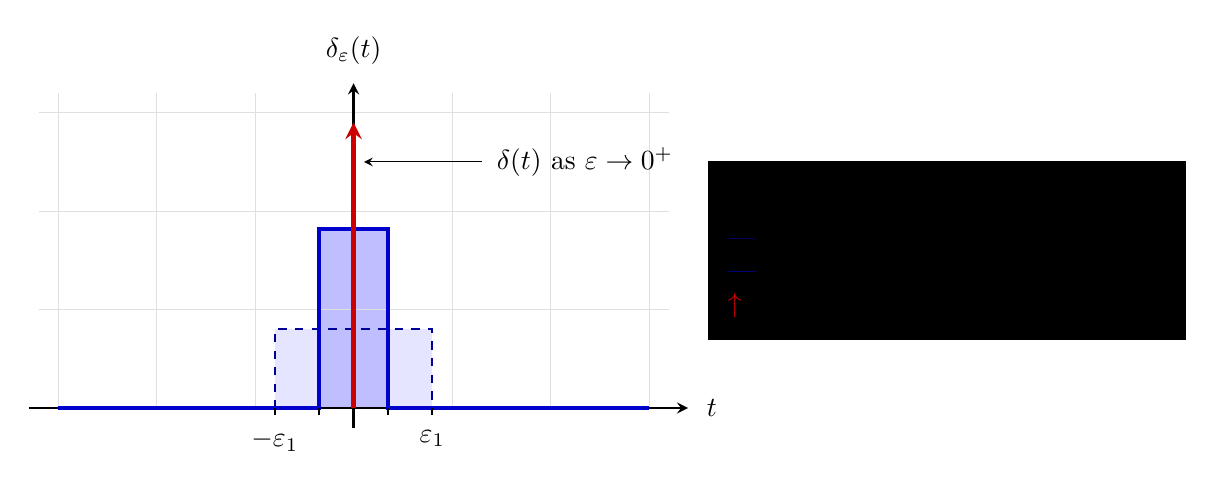
\begin{tikzpicture}[scale=1.25]
    % 1. Background fills
    \fill[blue!10] (-0.8, 0) rectangle (0.8, 0.8);
    \fill[blue!25] (-0.35, 0) rectangle (0.35, 1.82);

    % 2. Grid lines and axes
    \draw[help lines, gray!25] (-3.2, 0) grid (3.2, 3.2);
    \draw[->, >=stealth, thick] (-3.3, 0) -- (3.4, 0) node[right=3pt, black] {$t$};
    \draw[->, >=stealth, thick] (0, -0.2) -- (0, 3.3) node[above=3pt, black] {$\delta_\varepsilon(t)$};

    % 3. Primary plots
    \draw[thick, blue!60!black, dashed] (-3.0, 0) -- (-0.8, 0) -- (-0.8, 0.8) -- (0.8, 0.8) -- (0.8, 0) -- (3.0, 0);
    \draw[ultra thick, blue!80!black] (-3.0, 0) -- (-0.35, 0) -- (-0.35, 1.82) -- (0.35, 1.82) -- (0.35, 0) -- (3.0, 0);
    \draw[->, >=stealth, ultra thick, red!80!black] (0, 0) -- (0, 2.9);

    % 4. Labels, ticks, and single-node multiline legend
    \draw[thick] (-0.8, 0) -- (-0.8, -0.07) node[below=2pt, black] {$-\varepsilon_1$};
    \draw[thick] (0.8, 0) -- (0.8, -0.07) node[below=2pt, black] {$\varepsilon_1$};
    \draw[thick] (-0.35, 0) -- (-0.35, -0.07);
    \draw[thick] (0.35, 0) -- (0.35, -0.07);

    \draw[->, >=stealth, shorten >=2pt, black] (1.3, 2.5) -- (0.05, 2.5);
    \node[right=2pt, black, align=left] at (1.3, 2.5) {$\delta(t)$ as $\varepsilon \to 0^+$};

    \node[draw, fill=white, align=left, inner sep=7pt, anchor=west, black] at (3.6, 1.6) {%
        \textbf{Approximating $\delta(t)$}\\[4pt]
        {\color{blue!60!black}---} Wide pulse ($\varepsilon_1$): area $= 1$\\
        {\color{blue!80!black}---} Narrow pulse ($\varepsilon_2 < \varepsilon_1$): area $= 1$\\
        {\color{red!80!black}$\uparrow$} Limit $\delta(t)$: unit impulse at $t = 0$%
    };
\end{tikzpicture}
\end{center}

\textbf{Deriving the Sifting Property:} Suppose $f(t)$ is continuous near $t_0$. Integrating $f(t)\delta_\varepsilon(t - t_0)$ and applying the Mean Value Theorem for definite integrals gives
\[
    \int_{-\infty}^{\infty} f(t)\delta_\varepsilon(t - t_0)\,dt = \int_{t_0-\varepsilon}^{t_0+\varepsilon} f(t)\frac{1}{2\varepsilon}\,dt = f(c_\varepsilon)\int_{t_0-\varepsilon}^{t_0+\varepsilon} \frac{1}{2\varepsilon}\,dt = f(c_\varepsilon),
\]
for some $c_\varepsilon \in [t_0 - \varepsilon, t_0 + \varepsilon]$. Taking the limit as $\varepsilon \to 0^+$, continuity of $f$ forces $c_\varepsilon \to t_0$ and $f(c_\varepsilon) \to f(t_0)$. Thus:
\[
    \int_{-\infty}^{\infty} f(t)\delta(t - t_0)\,dt = f(t_0).
\]

\textbf{Deriving the Laplace Transform of $\delta(t - t_0)$:} Applying the sifting property with $f(t) = e^{-st}$ for $t_0 \ge 0$ (treating the lower limit $0$ as $0^-$ so that an impulse at $t_0 = 0$ is captured in full):
\[
    \mathcal{L}\{\delta(t - t_0)\}(s) = \int_{0^-}^{\infty} e^{-st}\delta(t - t_0)\,dt = e^{-st_0}.
\]
In particular, when $t_0 = 0$, $\mathcal{L}\{\delta(t)\}(s) = e^0 = 1$.

\textbf{Physical Interpretation of Symbolic IVPs:} Consider $m x'' + b x' + k x = I_0 \delta(t - t_0)$. Integrating both sides across the infinitesimally narrow interval $[t_0 - \varepsilon, t_0 + \varepsilon]$ yields
\[
    m\bigl(x'(t_0 + \varepsilon) - x'(t_0 - \varepsilon)\bigr) + b\bigl(x(t_0 + \varepsilon) - x(t_0 - \varepsilon)\bigr) + k\int_{t_0-\varepsilon}^{t_0+\varepsilon} x(t)\,dt = I_0.
\]
As $\varepsilon \to 0^+$, the position $x(t)$ remains continuous (so $x(t_0^+) - x(t_0^-) = 0$ and the integral of $x$ vanishes), leaving an instantaneous jump in momentum:
\[
    m\bigl(x'(t_0^+) - x'(t_0^-)\bigr) = I_0 \implies \Delta x'(t_0) = \frac{I_0}{m}.
\]
Hence, a Dirac delta forcing term leaves the solution $y(t)$ continuous at $t = t_0$ while inducing a jump discontinuity in its first derivative $y'(t)$ of size $I_0 / m$.

\subsection{Historical Context and Motivation}
The mathematical use of impulsive point-sources dates back to the nineteenth century in the work of Oliver Heaviside, who developed his ``operational calculus'' in the 1890s to solve transient problems in electrical telegraphy. Heaviside treated the derivative of the unit step function as a well-defined mathematical object, achieving exact physical predictions despite fierce criticism from pure mathematicians who noted that the step function is non-differentiable at the origin.

In 1926--1930, theoretical physicist Paul Dirac reintroduced and popularized the delta notation $\delta(x)$ in his foundational formulation of quantum mechanics, using it as a continuous analog of the Kronecker delta $\delta_{ij}$ to normalize continuous-spectrum eigenfunctions. It was not until the late 1940s that French mathematician Laurent Schwartz placed Heaviside's and Dirac's heuristic calculations on an airtight rigorous foundation through his \emph{Theory of Distributions} (for which he won the Fields Medal in 1950), demonstrating that $\delta$ is a continuous linear functional on the space of smooth compactly supported test functions.

\subsection{Key Formulas}
The essential formulas for mastering Section 7.9 are compiled below.

\renewcommand{\arraystretch}{1.5}
\begin{tabularx}{\textwidth}{>{\raggedright\arraybackslash}X >{$\displaystyle}c<{$} >{\raggedright\arraybackslash}X}
    \toprule
    \textbf{Concept / Property} & \textbf{Formula} & \textbf{Conditions / Notes} \\
    \midrule
    Sifting Property (Infinite Bounds) & \int_{-\infty}^{\infty} f(t)\delta(t - t_0)\,dt = f(t_0) & $f$ continuous at $t_0$. \\
    \addlinespace[4pt]
    Sifting Property (Finite Bounds) & \int_{a}^{b} f(t)\delta(t - t_0)\,dt = \begin{cases} f(t_0), & a < t_0 < b, \\ 0, & t_0 < a \text{ or } t_0 > b. \end{cases} & $f$ continuous on $[a,b]$; avoid $t_0 = a,b$. \\
    \addlinespace[4pt]
    Laplace Transform of Shifted Delta & \mathcal{L}\{\delta(t - t_0)\}(s) = e^{-t_0 s} & $t_0 \ge 0$; for $t_0 = 0$, $\mathcal{L}\{\delta(t)\} = 1$. \\
    \addlinespace[4pt]
    Laplace Transform of Product & \mathcal{L}\{f(t)\delta(t - t_0)\}(s) = f(t_0)e^{-t_0 s} & $t_0 \ge 0$ and $f$ continuous at $t_0$. \\
    \addlinespace[4pt]
    Second-Order Time Shift (Inverse) & \mathcal{L}^{-1}\{e^{-as} F(s)\} = u(t - a)f(t - a) & $a \ge 0$, where $f(t) = \mathcal{L}^{-1}\{F(s)\}$. \\
    \addlinespace[4pt]
    First-Order Frequency Shift & \mathcal{L}^{-1}\{F(s - a)\} = e^{at}f(t) & Used after completing the square. \\
    \addlinespace[4pt]
    Derivative Transforms & \mathcal{L}\{y'\}(s) = sY(s) - y(0) & $\mathcal{L}\{y''\}(s) = s^2 Y(s) - s y(0) - y'(0)$. \\
    \addlinespace[4pt]
    Impulse Response Function & a h'' + b h' + c h = \delta(t),\quad h(0)=0,\ h'(0)=0 & Gives $H(s) = \frac{1}{as^2 + bs + c}^{\vphantom{A}}$. \\
    \bottomrule
\end{tabularx}

\subsection{Prerequisites}
Before tackling Section 7.9, you must be fluent in the following prerequisite skills:
\begin{itemize}
    \item \textbf{Algebraic Manipulations:} Completing the square in quadratic denominators (e.g., $s^2 + 2s + 10 = (s+1)^2 + 3^2$) and partial fraction decomposition for distinct linear factors and irreducible quadratics.
    \item \textbf{Trigonometric Identities:} Angle-addition and subtraction formulas, specifically $\sin(\theta - n\pi)$ and $\sin(\theta - \pi/2) = -\cos\theta$, as well as evaluating $\sin$ and $\cos$ at standard multiples of $\pi/2$.
    \item \textbf{Core Calculus:} Improper integrals, the Mean Value Theorem for definite integrals, and the limit definition of continuity.
    \item \textbf{Earlier Laplace Transform Techniques (Sections 7.2--7.6):} Forward and inverse Laplace transforms of exponentials, polynomials, sines, and cosines; the first translation theorem ($s$-shifting); and the second translation theorem ($t$-shifting with the unit step function $u(t - a)$).
\end{itemize}

\newpage

\section{Detailed Homework Solutions}

\subsection{Problem 1}
\textbf{Original Problem:}
Evaluate the given integral.
\[
    \int_{-\infty}^{\infty} 7e^{2t}\delta(t)\,dt
\]

\textbf{Step-by-Step Solution:}
Identify the test function $f(t) = 7e^{2t}$ and the impulse location $t_0 = 0$, since $\delta(t) = \delta(t - 0)$. Because $f(t) = 7e^{2t}$ is continuous everywhere on $\R$ (and in particular at $t_0 = 0$), we apply the sifting property of the Dirac delta function:
\[
    \int_{-\infty}^{\infty} f(t)\delta(t - t_0)\,dt = f(t_0).
\]
Evaluating $f(t)$ at $t_0 = 0$:
\[
    \int_{-\infty}^{\infty} 7e^{2t}\delta(t)\,dt = f(0) = 7e^{2(0)} = 7e^0 = 7(1) = 7.
\]

\textbf{Final Answer:}
\[
    \int_{-\infty}^{\infty} 7e^{2t}\delta(t)\,dt = 7
\]

\subsection{Problem 2}
\textbf{Original Problem:}
Evaluate the given integral.
\[
    \int_{-\infty}^{\infty} 2e^{-3t}\delta(t + 4)\,dt
\]

\textbf{Step-by-Step Solution:}
Rewrite the shifted delta function in canonical form $\delta(t - t_0)$:
\[
    \delta(t + 4) = \delta\bigl(t - (-4)\bigr),
\]
so the impulse occurs at $t_0 = -4$. The multiplier function $f(t) = 2e^{-3t}$ is continuous everywhere on $\R$. Applying the sifting property:
\[
    \int_{-\infty}^{\infty} 2e^{-3t}\delta(t + 4)\,dt = f(-4) = 2e^{-3(-4)} = 2e^{12}.
\]

\textbf{Final Answer:}
\[
    \int_{-\infty}^{\infty} 2e^{-3t}\delta(t + 4)\,dt = 2e^{12}
\]

\subsection{Problem 3}
\textbf{Original Problem:}
Evaluate the given integral.
\[
    \int_{-1}^{1} (2\cos 3t)\delta(t)\,dt
\]

\textbf{Step-by-Step Solution:}
Here the integration bounds are finite: $[a, b] = [-1, 1]$. The impulse is located at $t_0 = 0$, which lies strictly inside the open interval $(-1, 1)$. Because $\delta(t) = 0$ for all $t \neq 0$, we have $\delta(t) = 0$ on $(-\infty, -1)$ and $(1, \infty)$, so the finite integral equals the full-line integral:
\[
    \int_{-1}^{1} (2\cos 3t)\delta(t)\,dt = \int_{-\infty}^{\infty} (2\cos 3t)\delta(t)\,dt.
\]
Since $f(t) = 2\cos(3t)$ is continuous at $t_0 = 0$, the sifting property gives
\[
    \int_{-1}^{1} (2\cos 3t)\delta(t)\,dt = f(0) = 2\cos\bigl(3(0)\bigr) = 2\cos(0) = 2(1) = 2.
\]

\textbf{Final Answer:}
\[
    \int_{-1}^{1} (2\cos 3t)\delta(t)\,dt = 2
\]

\subsection{Problem 4}
\textbf{Original Problem:}
Determine the Laplace transform of the given generalized function.
\[
    4\delta(t - 1)
\]

\textbf{Step-by-Step Solution:}
By definition of the Laplace transform (with $t_0 = 1 > 0$ inside $[0, \infty)$) and linearity of integration:
\[
    \mathcal{L}\{4\delta(t - 1)\}(s) = \int_{0}^{\infty} e^{-st}\bigl(4\delta(t - 1)\bigr)\,dt = 4\int_{0}^{\infty} e^{-st}\delta(t - 1)\,dt.
\]
Applying the sifting property at $t_0 = 1 \in (0, \infty)$ with continuous function $g(t) = e^{-st}$:
\[
    \mathcal{L}\{4\delta(t - 1)\}(s) = 4 e^{-s(1)} = 4e^{-s}.
\]

\textbf{Final Answer:}
\[
    \mathcal{L}\{4\delta(t - 1)\}(s) = 4e^{-s}
\]

\subsection{Problem 5}
\textbf{Original Problem:}
Determine the Laplace transform of the given generalized function.
\[
    6t^3\delta(t - 2)
\]

\textbf{Step-by-Step Solution:}
Using the definition of the Laplace transform, since $t_0 = 2 > 0$ lies strictly in $(0, \infty)$:
\[
    \mathcal{L}\{6t^3\delta(t - 2)\}(s) = \int_{0}^{\infty} e^{-st} \bigl(6t^3\delta(t - 2)\bigr)\,dt = \int_{0}^{\infty} \bigl(6t^3 e^{-st}\bigr)\delta(t - 2)\,dt.
\]
The integrand factor $f(t) = 6t^3 e^{-st}$ is continuous on $[0, \infty)$. Applying the sifting property at $t_0 = 2$:
\[
    \mathcal{L}\{6t^3\delta(t - 2)\}(s) = 6(2)^3 e^{-s(2)} = 6(8)e^{-2s} = 48e^{-2s}.
\]

\textbf{Final Answer:}
\[
    \mathcal{L}\{6t^3\delta(t - 2)\}(s) = 48e^{-2s}
\]

\subsection{Problem 6}
\textbf{Original Problem:}
Determine the Laplace transform of the given generalized function.
\[
    5e^{3t}\delta(t - 2)
\]

\textbf{Step-by-Step Solution:}
By the definition of the Laplace transform, with $t_0 = 2 \in (0, \infty)$:
\[
    \mathcal{L}\{5e^{3t}\delta(t - 2)\}(s) = \int_{0}^{\infty} e^{-st}\bigl(5e^{3t}\bigr)\delta(t - 2)\,dt.
\]
Since $f(t) = 5e^{3t}e^{-st} = 5e^{(3-s)t}$ is continuous at $t_0 = 2$, the sifting property yields
\[
    \mathcal{L}\{5e^{3t}\delta(t - 2)\}(s) = 5e^{3(2)}e^{-s(2)} = 5e^{6}e^{-2s} = 5e^{6 - 2s}.
\]

\textbf{Final Answer:}
\[
    \mathcal{L}\{5e^{3t}\delta(t - 2)\}(s) = 5e^{6 - 2s}
\]

\subsection{Problem 7}
\textbf{Original Problem:}
Solve the given symbolic initial value problem.
\[
    y'' + 2y' + 10y = 3\delta(t - \pi); \quad y(0) = 2,\quad y'(0) = 4
\]
What is the Laplace transform $Y(s)$ of the solution $y(t)$? Solve the given symbolic initial value problem.

\textbf{Step-by-Step Solution:}
\textbf{Step 1: Take the Laplace transform of both sides.}
Let $Y(s) = \mathcal{L}\{y(t)\}(s)$. Using the derivative rules $\mathcal{L}\{y''\} = s^2 Y(s) - sy(0) - y'(0)$ and $\mathcal{L}\{y'\} = sY(s) - y(0)$, along with $\mathcal{L}\{\delta(t - \pi)\} = e^{-\pi s}$:
\[
    \bigl(s^2 Y(s) - s(2) - 4\bigr) + 2\bigl(sY(s) - 2\bigr) + 10Y(s) = 3e^{-\pi s}.
\]
Group the $Y(s)$ terms and constant/linear $s$ terms:
\[
    (s^2 + 2s + 10)Y(s) - 2s - 4 - 4 = 3e^{-\pi s} \implies (s^2 + 2s + 10)Y(s) = 2s + 8 + 3e^{-\pi s}.
\]
Dividing by $s^2 + 2s + 10$ gives $Y(s)$:
\[
    Y(s) = \frac{2s + 8 + 3e^{-\pi s}}{s^2 + 2s + 10}.
\]

\textbf{Step 2: Complete the square and rewrite $Y(s)$ in standard inverse-transform forms.}
Complete the square in the denominator:
\[
    s^2 + 2s + 10 = (s^2 + 2s + 1) + 9 = (s + 1)^2 + 3^2.
\]
Split the numerator $2s + 8$ in terms of $(s + 1)$:
\[
    2s + 8 = 2(s + 1) + 6 = 2(s + 1) + 2(3).
\]
Therefore,
\[
    Y(s) = 2\cdot \frac{s + 1}{(s + 1)^2 + 3^2} + 2\cdot \frac{3}{(s + 1)^2 + 3^2} + e^{-\pi s}\cdot \frac{3}{(s + 1)^2 + 3^2}.
\]

\textbf{Step 3: Take the inverse Laplace transform.}
Using the first translation theorem, $\mathcal{L}^{-1}\left\{\frac{s+1}{(s+1)^2+3^2}\right\} = e^{-t}\cos(3t)$ and $\mathcal{L}^{-1}\left\{\frac{3}{(s+1)^2+3^2}\right\} = e^{-t}\sin(3t)$. For the third term, apply the second translation theorem $\mathcal{L}^{-1}\{e^{-\pi s}F(s)\} = u(t - \pi)f(t - \pi)$:
\[
    y(t) = 2e^{-t}\cos(3t) + 2e^{-t}\sin(3t) + u(t - \pi)e^{-(t - \pi)}\sin\bigl(3(t - \pi)\bigr).
\]
Note that $\sin(3t - 3\pi) = \sin(3t)\cos(3\pi) - \cos(3t)\sin(3\pi) = -\sin(3t)$, so the shifted term can equivalently be written as $-u(t - \pi)e^{\pi - t}\sin(3t)$.

\textbf{Final Answer:}
\[
    Y(s) = \frac{2s + 8 + 3e^{-\pi s}}{s^2 + 2s + 10}
\]
\[
    y(t) = 2e^{-t}\cos(3t) + 2e^{-t}\sin(3t) + u(t - \pi)e^{-(t - \pi)}\sin\bigl(3(t - \pi)\bigr)
\]

\subsection{Problem 8}
\textbf{Original Problem:}
Solve the given symbolic initial value problem.
\[
    y'' + 2y' - 3y = \delta(t - 4) - \delta(t - 6); \quad y(0) = 8,\quad y'(0) = -4
\]

\textbf{Step-by-Step Solution:}
\textbf{Step 1: Take the Laplace transform.}
Let $Y(s) = \mathcal{L}\{y(t)\}(s)$. Transforming both sides with $y(0) = 8$ and $y'(0) = -4$:
\[
    \bigl(s^2 Y(s) - 8s - (-4)\bigr) + 2\bigl(sY(s) - 8\bigr) - 3Y(s) = e^{-4s} - e^{-6s}.
\]
Simplify and collect $Y(s)$:
\[
    (s^2 + 2s - 3)Y(s) - 8s + 4 - 16 = e^{-4s} - e^{-6s} \implies (s + 3)(s - 1)Y(s) = 8s + 12 + e^{-4s} - e^{-6s}.
\]
Thus,
\[
    Y(s) = \frac{8s + 12}{(s + 3)(s - 1)} + \bigl(e^{-4s} - e^{-6s}\bigr)\frac{1}{(s + 3)(s - 1)}.
\]

\textbf{Step 2: Perform partial fraction decomposition.}
First, decompose $\frac{8s + 12}{(s + 3)(s - 1)}$:
\[
    \frac{8s + 12}{(s + 3)(s - 1)} = \frac{A}{s - 1} + \frac{B}{s + 3} \implies 8s + 12 = A(s + 3) + B(s - 1).
\]
\begin{itemize}
    \item Setting $s = 1$: $8(1) + 12 = 4A \implies 20 = 4A \implies A = 5$.
    \item Setting $s = -3$: $8(-3) + 12 = -4B \implies -12 = -4B \implies B = 3$.
\end{itemize}
Next, decompose $\frac{1}{(s + 3)(s - 1)}$:
\[
    \frac{1}{(s + 3)(s - 1)} = \frac{C}{s - 1} + \frac{D}{s + 3} \implies 1 = C(s + 3) + D(s - 1).
\]
\begin{itemize}
    \item Setting $s = 1$: $1 = 4C \implies C = \frac{1}{4}$.
    \item Setting $s = -3$: $1 = -4D \implies D = -\frac{1}{4}$.
\end{itemize}
Substituting both decompositions into $Y(s)$ gives
\[
    Y(s) = \frac{5}{s - 1} + \frac{3}{s + 3} + \frac{1}{4}e^{-4s}\left(\frac{1}{s - 1} - \frac{1}{s + 3}\right) - \frac{1}{4}e^{-6s}\left(\frac{1}{s - 1} - \frac{1}{s + 3}\right).
\]

\textbf{Step 3: Take the inverse Laplace transform.}
Using $\mathcal{L}^{-1}\left\{\frac{1}{s - a}\right\} = e^{at}$ and the $t$-shifting property:
\[
    y(t) = 5e^{t} + 3e^{-3t} + \frac{1}{4}u(t - 4)\bigl(e^{t - 4} - e^{-3(t - 4)}\bigr) - \frac{1}{4}u(t - 6)\bigl(e^{t - 6} - e^{-3(t - 6)}\bigr).
\]

\textbf{Final Answer:}
\[
    y(t) = 5e^{t} + 3e^{-3t} + \frac{1}{4}u(t - 4)\bigl(e^{t - 4} - e^{-3(t - 4)}\bigr) - \frac{1}{4}u(t - 6)\bigl(e^{t - 6} - e^{-3(t - 6)}\bigr)
\]

\subsection{Problem 9}
\textbf{Original Problem:}
Solve the given symbolic initial value problem.
\[
    y'' - y' - 2y = 3\delta(t - 3) + e^{t}; \quad y(0) = 0,\quad y'(0) = 3
\]

\textbf{Step-by-Step Solution:}
\textbf{Step 1: Take the Laplace transform.}
With $y(0) = 0$, $y'(0) = 3$, $\mathcal{L}\{\delta(t - 3)\} = e^{-3s}$, and $\mathcal{L}\{e^{t}\} = \frac{1}{s - 1}$:
\[
    \bigl(s^2 Y(s) - 0 - 3\bigr) - \bigl(sY(s) - 0\bigr) - 2Y(s) = 3e^{-3s} + \frac{1}{s - 1}.
\]
Factor the left-hand side:
\[
    (s^2 - s - 2)Y(s) = 3 + \frac{1}{s - 1} + 3e^{-3s}.
\]
Combine $3 + \frac{1}{s - 1} = \frac{3(s - 1) + 1}{s - 1} = \frac{3s - 2}{s - 1}$ and factor $s^2 - s - 2 = (s - 2)(s + 1)$:
\[
    Y(s) = \frac{3s - 2}{(s - 1)(s - 2)(s + 1)} + \frac{3e^{-3s}}{(s - 2)(s + 1)}.
\]

\textbf{Step 2: Perform partial fraction decomposition.}
First, decompose $F_1(s) = \frac{3s - 2}{(s - 1)(s - 2)(s + 1)}$:
\[
    \frac{3s - 2}{(s - 1)(s - 2)(s + 1)} = \frac{A}{s - 1} + \frac{B}{s - 2} + \frac{C}{s + 1}.
\]
Multiply through by $(s - 1)(s - 2)(s + 1)$:
\[
    3s - 2 = A(s - 2)(s + 1) + B(s - 1)(s + 1) + C(s - 1)(s - 2).
\]
\begin{itemize}
    \item Setting $s = 1$: $3(1) - 2 = A(-1)(2) \implies 1 = -2A \implies A = -\frac{1}{2}$.
    \item Setting $s = 2$: $3(2) - 2 = B(1)(3) \implies 4 = 3B \implies B = \frac{4}{3}$.
    \item Setting $s = -1$: $3(-1) - 2 = C(-2)(-3) \implies -5 = 6C \implies C = -\frac{5}{6}$.
\end{itemize}
Second, decompose $F_2(s) = \frac{3}{(s - 2)(s + 1)}$:
\[
    \frac{3}{(s - 2)(s + 1)} = \frac{D}{s - 2} + \frac{E}{s + 1} \implies 3 = D(s + 1) + E(s - 2).
\]
\begin{itemize}
    \item Setting $s = 2$: $3 = 3D \implies D = 1$.
    \item Setting $s = -1$: $3 = -3E \implies E = -1$.
\end{itemize}
Therefore,
\[
    Y(s) = -\frac{1}{2}\cdot\frac{1}{s - 1} + \frac{4}{3}\cdot\frac{1}{s - 2} - \frac{5}{6}\cdot\frac{1}{s + 1} + e^{-3s}\left(\frac{1}{s - 2} - \frac{1}{s + 1}\right).
\]

\textbf{Step 3: Take the inverse Laplace transform.}
Inverting term by term with the second translation theorem for the $e^{-3s}$ factor:
\[
    y(t) = -\frac{1}{2}e^{t} + \frac{4}{3}e^{2t} - \frac{5}{6}e^{-t} + u(t - 3)\bigl(e^{2(t - 3)} - e^{-(t - 3)}\bigr).
\]

\textbf{Final Answer:}
\[
    y(t) = -\frac{1}{2}e^{t} + \frac{4}{3}e^{2t} - \frac{5}{6}e^{-t} + u(t - 3)\bigl(e^{2(t - 3)} - e^{-(t - 3)}\bigr)
\]

\subsection{Problem 10}
\textbf{Original Problem:}
Solve the given symbolic initial value problem and sketch a graph of the solution.
\[
    y'' + y = 2\delta\left(t - \frac{\pi}{2}\right); \quad y(0) = 0,\quad y'(0) = 4
\]
(Multiple-choice graph options A, B, C, and D on $[0, 2\pi] \times [-7, 7]$.)

\textbf{Step-by-Step Solution:}
\textbf{Step 1: Solve the symbolic IVP via Laplace transforms.}
Applying $\mathcal{L}$ to both sides with $y(0) = 0$ and $y'(0) = 4$:
\[
    \bigl(s^2 Y(s) - 0 - 4\bigr) + Y(s) = 2e^{-\frac{\pi}{2}s} \implies (s^2 + 1)Y(s) = 4 + 2e^{-\frac{\pi}{2}s}.
\]
Divide by $s^2 + 1$:
\[
    Y(s) = \frac{4}{s^2 + 1} + 2e^{-\frac{\pi}{2}s}\cdot \frac{1}{s^2 + 1}.
\]
Inverting using $\mathcal{L}^{-1}\left\{\frac{1}{s^2 + 1}\right\} = \sin t$ and the second translation theorem:
\[
    y(t) = 4\sin t + 2u\left(t - \frac{\pi}{2}\right)\sin\left(t - \frac{\pi}{2}\right).
\]
Using the identity $\sin\left(t - \frac{\pi}{2}\right) = -\cos t$, we can also express $y(t)$ piecewise:
\[
    y(t) = \begin{cases} 4\sin t, & 0 \le t < \dfrac{\pi}{2}, \\[6pt] 4\sin t - 2\cos t, & t \ge \dfrac{\pi}{2}. \end{cases}
\]

\textbf{Step 2: Analyze key geometric features to identify the graph.}
\begin{itemize}
    \item At $t = 0$: $y(0) = 0$ and $y'(0) = 4$. (Eliminates Graph A, which starts at $y(0) = -4$.)
    \item At $t = \frac{\pi}{2}$: $y(\pi/2) = 4\sin(\pi/2) = 4$. Notice the derivative just before the impulse is $y'((\pi/2)^-) = 4\cos(\pi/2) = 0$, whereas just after the impulse it jumps by $+2$ to $y'((\pi/2)^+) = 4\cos(\pi/2) + 2\sin(\pi/2) = 2 > 0$. Thus, the curve exhibits a sharp upward corner at $(\pi/2, 4)$ and continues rising above $4$.
    \item For $t > \frac{\pi}{2}$: $y(t) = 4\sin t - 2\cos t$ has amplitude $\sqrt{4^2 + (-2)^2} = \sqrt{20} = 2\sqrt{5} \approx 4.47$.
    \item At $t = \pi$: $y(\pi) = 4\sin\pi - 2\cos\pi = 2$. At $t = 2\pi$: $y(2\pi) = 4\sin(2\pi) - 2\cos(2\pi) = -2$.
\end{itemize}
Graph \textbf{B} starts at $(0, 0)$, reaches $(\pi/2, 4)$ with an upward kink to a peak of $\approx 4.47$, passes through $(\pi, 2)$, reaches a minimum of $\approx -4.47$, and ends at $(2\pi, -2)$. (By contrast, Graph C overshoots to nearly $6$, and Graph D drops immediately after $\pi/2$ through $(\pi, 0)$.)

\begin{center}
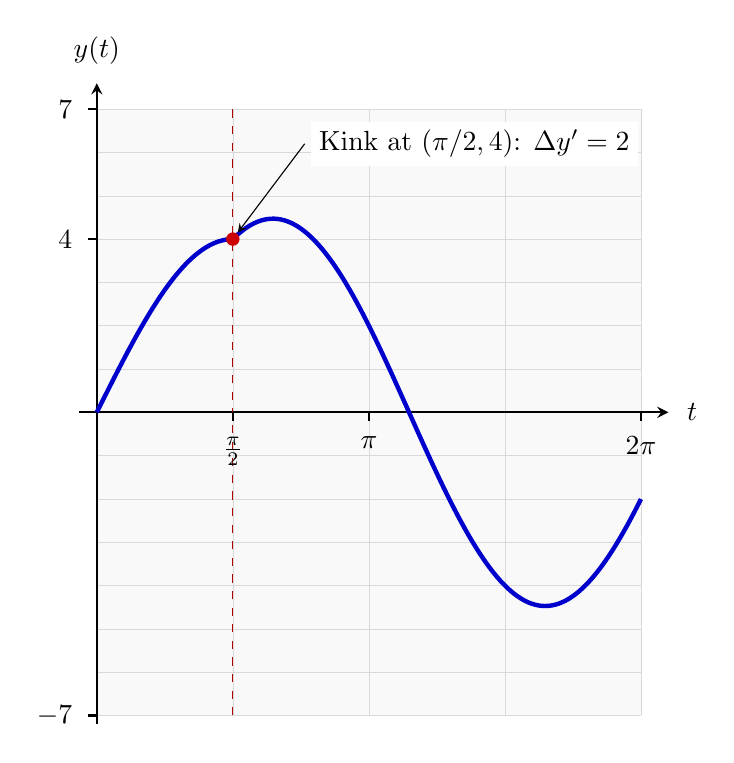
\begin{tikzpicture}[scale=1.1]
    % 1. Background fill
    \fill[gray!5] (0, -3.5) rectangle (6.283, 3.5);

    % 2. Grid lines and axes (y scaled by 0.5 so 7 -> 3.5)
    \draw[help lines, gray!30] (0, -3.5) grid[xstep=1.5708, ystep=0.5] (6.283, 3.5);
    \draw[->, >=stealth, thick] (-0.2, 0) -- (6.6, 0) node[right=3pt, black] {$t$};
    \draw[->, >=stealth, thick] (0, -3.6) -- (0, 3.8) node[above=3pt, black] {$y(t)$};

    % 3. Primary plot (y divided by 2 for clean vertical proportions)
    \draw[ultra thick, blue!80!black, domain=0:1.5708, samples=60] plot (\x, {2*sin(\x r)});
    \draw[ultra thick, blue!80!black, domain=1.5708:6.2832, samples=120] plot (\x, {2*sin(\x r) - cos(\x r)});
    \draw[dashed, red!70!black] (1.5708, -3.5) -- (1.5708, 3.5);

    % 4. Ticks, nodes, and off-axis callout
    \draw[thick] (1.5708, 0) -- (1.5708, -0.1) node[below=2pt, black] {$\frac{\pi}{2}$};
    \draw[thick] (3.1416, 0) -- (3.1416, -0.1) node[below=2pt, black] {$\pi$};
    \draw[thick] (6.2832, 0) -- (6.2832, -0.1) node[below=2pt, black] {$2\pi$};
    \draw[thick] (0, 2) -- (-0.1, 2) node[left=2pt, black] {$4$};
    \draw[thick] (0, 3.5) -- (-0.1, 3.5) node[left=2pt, black] {$7$};
    \draw[thick] (0, -3.5) -- (-0.1, -3.5) node[left=2pt, black] {$-7$};

    \fill[red!80!black] (1.5708, 2) circle (2.2pt);
    \draw[->, >=stealth, shorten >=3pt, black] (2.4, 3.1) -- (1.5708, 2);
    \node[right=2pt, black, align=left, fill=white, inner sep=3pt] at (2.4, 3.1) {Kink at $(\pi/2, 4)$: $\Delta y' = 2$};
\end{tikzpicture}
\end{center}

\textbf{Final Answer:}
\[
    y(t) = 4\sin t + 2u\left(t - \frac{\pi}{2}\right)\sin\left(t - \frac{\pi}{2}\right) \quad \text{(equivalently } 4\sin t - 2u\left(t - \frac{\pi}{2}\right)\cos t\text{)}, \quad \text{Graph: \textbf{B}}
\]

\subsection{Problem 11}
\textbf{Original Problem:}
Find the impulse response function $h(t)$ by using the fact that $h(t)$ is the solution to the symbolic initial value problem with $g(t) = \delta(t)$ and zero initial conditions.
\[
    y'' + 2y' + 10y = g(t)
\]

\textbf{Step-by-Step Solution:}
Set $g(t) = \delta(t)$, $y(t) = h(t)$, $h(0) = 0$, and $h'(0) = 0$:
\[
    h'' + 2h' + 10h = \delta(t); \quad h(0) = 0,\quad h'(0) = 0.
\]
Taking the Laplace transform of both sides with $H(s) = \mathcal{L}\{h(t)\}(s)$ and $\mathcal{L}\{\delta(t)\} = 1$:
\[
    (s^2 + 2s + 10)H(s) = 1 \implies H(s) = \frac{1}{s^2 + 2s + 10}.
\]
Complete the square in the denominator:
\[
    s^2 + 2s + 10 = (s + 1)^2 + 9 = (s + 1)^2 + 3^2.
\]
Multiply and divide by $3$ to match the sine template:
\[
    H(s) = \frac{1}{3}\cdot \frac{3}{(s + 1)^2 + 3^2}.
\]
Applying the first translation theorem to invert:
\[
    h(t) = \frac{1}{3}e^{-t}\sin(3t) \quad (t \ge 0).
\]

\textbf{Final Answer:}
\[
    h(t) = \frac{1}{3}e^{-t}\sin(3t)
\]

\subsection{Problem 12}
\textbf{Original Problem:}
Find the impulse response function $h(t)$ by using the fact that $h(t)$ is the solution to the symbolic initial value problem with $g(t) = \delta(t)$ and zero initial conditions.
\[
    y'' - 6y' + 34y = g(t)
\]

\textbf{Step-by-Step Solution:}
Set up the impulse response IVP:
\[
    h'' - 6h' + 34h = \delta(t); \quad h(0) = 0,\quad h'(0) = 0.
\]
Take the Laplace transform:
\[
    (s^2 - 6s + 34)H(s) = 1 \implies H(s) = \frac{1}{s^2 - 6s + 34}.
\]
Complete the square in the denominator:
\[
    s^2 - 6s + 34 = (s^2 - 6s + 9) + 25 = (s - 3)^2 + 5^2.
\]
Adjust for the numerator factor $b = 5$:
\[
    H(s) = \frac{1}{5}\cdot \frac{5}{(s - 3)^2 + 5^2}.
\]
Inverting via the first translation theorem yields
\[
    h(t) = \frac{1}{5}e^{3t}\sin(5t) \quad (t \ge 0).
\]

\textbf{Final Answer:}
\[
    h(t) = \frac{1}{5}e^{3t}\sin(5t)
\]

\subsection{Problem 13}
\textbf{Original Problem:}
Find the impulse response function $h(t)$ by using the fact that $h(t)$ is the solution to the symbolic initial value problem with $g(t) = \delta(t)$ and zero initial conditions.
\[
    y'' - 25y = g(t)
\]

\textbf{Step-by-Step Solution:}
Formulate the impulse response IVP:
\[
    h'' - 25h = \delta(t); \quad h(0) = 0,\quad h'(0) = 0.
\]
Take the Laplace transform:
\[
    (s^2 - 25)H(s) = 1 \implies H(s) = \frac{1}{s^2 - 25} = \frac{1}{(s - 5)(s + 5)}.
\]
Decompose into partial fractions:
\[
    \frac{1}{(s - 5)(s + 5)} = \frac{A}{s - 5} + \frac{B}{s + 5} \implies 1 = A(s + 5) + B(s - 5).
\]
\begin{itemize}
    \item Setting $s = 5$: $1 = 10A \implies A = \frac{1}{10}$.
    \item Setting $s = -5$: $1 = -10B \implies B = -\frac{1}{10}$.
\end{itemize}
Thus,
\[
    H(s) = \frac{1}{10}\left(\frac{1}{s - 5} - \frac{1}{s + 5}\right).
\]
Inverting term by term:
\[
    h(t) = \frac{1}{10}\left(e^{5t} - e^{-5t}\right) = \frac{1}{5}\sinh(5t) \quad (t \ge 0).
\]

\textbf{Final Answer:}
\[
    h(t) = \frac{1}{10}\left(e^{5t} - e^{-5t}\right)
\]

\subsection{Problem 14}
\textbf{Original Problem:}
A mass attached to a spring is released from rest $4\text{ m}$ below the equilibrium position for the mass-spring system and begins to vibrate. After $\frac{\pi}{2}\text{ sec}$, the mass is struck by a hammer exerting an impulse on the mass. The system is governed by the symbolic initial value problem below, where $x(t)$ denotes the displacement from equilibrium at time $t$. What happens to the mass after it is struck?
\[
    \frac{d^2 x}{dt^2} + 225x = -60\delta\left(t - \frac{\pi}{2}\right), \quad x(0) = 4,\quad x'(0) = 0
\]
Options:
\begin{enumerate}[label=\Alph*.]
    \item The mass moves downward since $x(t) < 0$ for values of $t$ slightly larger than $\frac{\pi}{2}$.
    \item The mass remains stopped at $x(t) = 0$, for $t > \frac{\pi}{2}$.
    \item The mass moves upward since $x(t) > 0$ for values of $t$ slightly larger than $\frac{\pi}{2}$.
    \item It cannot be determined since $x(t)$ is undefined for $t > \frac{\pi}{2}$.
\end{enumerate}

\textbf{Step-by-Step Solution:}
\textbf{Step 1: Solve the symbolic IVP for $x(t)$.}
Let $X(s) = \mathcal{L}\{x(t)\}(s)$. Taking the Laplace transform with $x(0) = 4$ and $x'(0) = 0$:
\[
    \bigl(s^2 X(s) - 4s - 0\bigr) + 225 X(s) = -60 e^{-\frac{\pi}{2}s} \implies (s^2 + 15^2)X(s) = 4s - 60 e^{-\frac{\pi}{2}s}.
\]
Divide by $s^2 + 15^2$:
\[
    X(s) = 4\cdot\frac{s}{s^2 + 15^2} - 4e^{-\frac{\pi}{2}s}\cdot\frac{15}{s^2 + 15^2}.
\]
Take the inverse Laplace transform:
\[
    x(t) = 4\cos(15t) - 4u\left(t - \frac{\pi}{2}\right)\sin\left(15\left(t - \frac{\pi}{2}\right)\right).
\]

\textbf{Step 2: Simplify $x(t)$ for $t > \frac{\pi}{2}$.}
For $t > \frac{\pi}{2}$, $u\left(t - \frac{\pi}{2}\right) = 1$, and we expand the shifted sine term:
\[
    15\left(t - \frac{\pi}{2}\right) = 15t - \frac{15\pi}{2} = 15t - \left(6\pi + \frac{3\pi}{2}\right).
\]
Using the $2\pi$-periodicity of sine and the subtraction identity:
\[
    \sin\left(15t - \frac{3\pi}{2}\right) = \sin(15t)\cos\left(\frac{3\pi}{2}\right) - \cos(15t)\sin\left(\frac{3\pi}{2}\right) = 0 - \cos(15t)(-1) = \cos(15t).
\]
Substituting this back into $x(t)$ for $t > \frac{\pi}{2}$:
\[
    x(t) = 4\cos(15t) - 4\cos(15t) = 0 \quad \text{for all } t > \frac{\pi}{2}.
\]
Physically, at $t = \frac{\pi}{2}$, the mass passes through equilibrium ($x(\pi/2) = 4\cos(15\pi/2) = 0$) with velocity $x'((\pi/2)^-) = -60\sin(15\pi/2) = +60\text{ m/s}$, and the hammer delivers an exact canceling impulse of $-60$, bringing both position and velocity to zero simultaneously.

\begin{center}
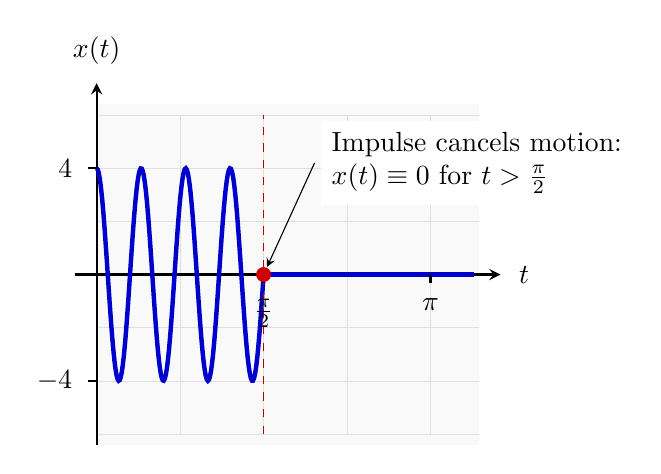
\begin{tikzpicture}[scale=1.35]
    % 1. Background fill
    \fill[gray!5] (0, -1.6) rectangle (3.6, 1.6);

    % 2. Grid and axes (vertical scale 1 unit = 4 m so 4 m -> 1.0)
    \draw[help lines, gray!25] (0, -1.5) grid[xstep=0.7854, ystep=0.5] (3.6, 1.5);
    \draw[->, >=stealth, thick] (-0.2, 0) -- (3.8, 0) node[right=3pt, black] {$t$};
    \draw[->, >=stealth, thick] (0, -1.6) -- (0, 1.8) node[above=3pt, black] {$x(t)$};

    % 3. Primary plot: cos(15t) on [0, pi/2], then 0 on [pi/2, 3.6]
    \draw[ultra thick, blue!80!black, domain=0:1.5708, samples=160] plot (\x, {cos(15*\x r)});
    \draw[ultra thick, blue!80!black] (1.5708, 0) -- (3.55, 0);
    \draw[dashed, red!70!black] (1.5708, -1.5) -- (1.5708, 1.5);

    % 4. Ticks and callout
    \draw[thick] (1.5708, 0) -- (1.5708, -0.08) node[below=2pt, black] {$\frac{\pi}{2}$};
    \draw[thick] (3.1416, 0) -- (3.1416, -0.08) node[below=2pt, black] {$\pi$};
    \draw[thick] (0, 1.0) -- (-0.08, 1.0) node[left=2pt, black] {$4$};
    \draw[thick] (0, -1.0) -- (-0.08, -1.0) node[left=2pt, black] {$-4$};

    \fill[red!80!black] (1.5708, 0) circle (2pt);
    \draw[->, >=stealth, shorten >=3pt, black] (2.05, 1.05) -- (1.5708, 0);
    \node[right=2pt, black, align=left, fill=white, inner sep=4pt] at (2.05, 1.05) {Impulse cancels motion:\\$x(t) \equiv 0$ for $t > \frac{\pi}{2}$};
\end{tikzpicture}
\end{center}

\textbf{Final Answer:}
\textbf{B.} The mass remains stopped at $x(t) = 0$, for $t > \frac{\pi}{2}$.

\subsection{Problem 15}
\textbf{Original Problem:}
The Dirac delta function $\delta(t)$ may also be characterized by the following two properties:
\[
    \delta(t) = \begin{cases} 0, & t \neq 0, \\ \text{``infinite,''} & t = 0, \end{cases} \quad \text{and} \quad \int_{-\infty}^{\infty} \delta(t)\,dt = 1.
\]
Formally using the mean value theorem for definite integrals, verify that if $f(t)$ is continuous, then the above properties imply $\int_{-\infty}^{\infty} f(t)\delta(t)\,dt = f(0)$, by completing items (1)--(10) and the interval/value boxes.

\textbf{Step-by-Step Solution:}
\begin{enumerate}
    \item \textbf{Statement of the Mean Value Theorem for Definite Integrals:} If $f(t)$ is continuous on $[a, b]$, there exists a value $c$ in the interval \textbf{(1) $[a, b]$} such that
    \[
        f(c) = \text{\textbf{(2)} } \frac{1}{b - a}\int_{a}^{b} f(t)\,dt.
    \]

    \item \textbf{Splitting the Integral:} Using additivity of the integral at $-\varepsilon$ and $\varepsilon$ ($\varepsilon > 0$):
    \[
        \int_{-\infty}^{\infty} f(t)\delta(t)\,dt = \int_{-\infty}^{\boxed{-\varepsilon}} f(t)\delta(t)\,dt + \int_{\boxed{-\varepsilon}}^{\boxed{\varepsilon}} f(t)\delta(t)\,dt + \int_{\boxed{\varepsilon}}^{\infty} f(t)\delta(t)\,dt.
    \]

    \item \textbf{Vanishing Tail Integrals:} On $(-\infty, -\varepsilon]$ and $[\varepsilon, \infty)$, $t \neq 0$, so $\delta(t) = 0$ everywhere on those intervals. Hence, the \textbf{(3) first and third} integrals both evaluate to $\boxed{0}$.

    \item \textbf{Applying the Generalized Mean Value Theorem:} Since \textbf{(4) $f$ is continuous}, and $\delta(t) \ge 0$ is integrable, there exists a value $c$ in the interval \textbf{(5) $[-\varepsilon, \varepsilon]$} such that
    \[
        \int_{-\varepsilon}^{\varepsilon} f(t)\delta(t)\,dt = \text{\textbf{(6)} } f(c)\int_{-\varepsilon}^{\varepsilon} \delta(t)\,dt.
    \]

    \item \textbf{Taking the Small-$\varepsilon$ Limit:} As $\varepsilon$ decreases, the width of the interval \textbf{(7) $[-\varepsilon, \varepsilon]$} decreases ($2\varepsilon \to 0$) and $c$ is squeezed toward $0$. For suitably small $\varepsilon$, \textbf{(8) $f$ will be approximately constant} over $[-\varepsilon, \varepsilon]$, leading to the relation \textbf{(9) $f(-\varepsilon) \approx f(0) \approx f(\varepsilon)$} (so $f(c) \to f(0)$ as $\varepsilon \to 0^+$).

    \item \textbf{Final Evaluation:} Because $\delta(t) = 0$ outside $[-\varepsilon, \varepsilon]$, the total unit mass is concentrated in $[-\varepsilon, \varepsilon]$. Since \textbf{(10) $\int_{-\varepsilon}^{\varepsilon} \delta(t)\,dt$} $= \boxed{1}$ and $\varepsilon > 0$ can be chosen arbitrarily small, we conclude $\int_{-\infty}^{\infty} f(t)\delta(t)\,dt = f(0)$.
\end{enumerate}

\textbf{Final Answer Summary:}
\begin{itemize}
    \item \textbf{(1)} $[a, b]$, \quad \textbf{(2)} $\frac{1}{b - a}\int_{a}^{b} f(t)\,dt$, \quad \textbf{Integral Bounds:} $-\varepsilon$, $-\varepsilon$, $\varepsilon$, $\varepsilon$, \quad \textbf{(3)} first and third, \quad \textbf{Box:} $0$
    \item \textbf{(4)} $f$ is continuous, \quad \textbf{(5)} $[-\varepsilon, \varepsilon]$, \quad \textbf{(6)} $f(c)\int_{-\varepsilon}^{\varepsilon} \delta(t)\,dt$, \quad \textbf{(7)} $[-\varepsilon, \varepsilon]$, \quad \textbf{(8)} $f$ will be approximately constant
    \item \textbf{(9)} $f(-\varepsilon) \approx f(0) \approx f(\varepsilon)$, \quad \textbf{(10)} $\int_{-\varepsilon}^{\varepsilon} \delta(t)\,dt$, \quad \textbf{Box:} $1$
\end{itemize}

\newpage

\section{In-Depth Analysis of Problems and Techniques}

\subsection{Problem Types and General Approach}
\begin{description}
    \item[Type 1: Direct Sifting Integral Evaluations (Problems 1, 2, 3)]
    Identify the impulse center $t_0$ by setting the argument of $\delta(\cdot)$ to zero. Check whether $t_0$ lies strictly inside the interval of integration $(a, b)$. If $t_0 \in (a, b)$ and the remaining integrand $f(t)$ is continuous at $t_0$, the integral immediately collapses to $f(t_0)$; if $t_0 \notin [a, b]$, the integral is $0$.

    \item[Type 2: Laplace Transforms of Generalized Functions (Problems 4, 5, 6)]
    Write the Laplace transform integral $\int_0^{\infty} e^{-st} f(t)\delta(t - t_0)\,dt$. Verify that $t_0 \ge 0$, treat $f(t)e^{-st}$ as the continuous test function, and evaluate it at $t = t_0$ to obtain $f(t_0)e^{-t_0 s}$. Note that any time-dependent prefactor $f(t)$ multiplying $\delta(t - t_0)$ collapses to the constant $f(t_0)$ before transforming.

    \item[Type 3: Symbolic IVPs with Complex Characteristic Roots (Problems 7, 10)]
    Apply the Laplace transform to convert the differential equation into an algebraic equation for $Y(s)$. Separate the forcing exponential $e^{-t_0 s}$ from the initial-condition polynomial. Complete the square in the quadratic denominator $(s - a)^2 + b^2$, rewrite the numerator in terms of $(s - a)$ and $b$, and invert using the first and second translation theorems.

    \item[Type 4: Symbolic IVPs with Real Distinct Roots and Mixed Forcing (Problems 8, 9)]
    Transform the ODE, separating standard rational terms (from initial conditions and ordinary forcing like $e^t$) from exponential-weighted rational terms (from $\delta(t - t_0)$). Perform partial fraction decomposition separately on the unshifted and shifted transfer terms, and invert into exponentials and step-shifted exponentials.

    \item[Type 5: Impulse Response Function Determination (Problems 11, 12, 13)]
    Set $g(t) = \delta(t)$ and impose zero initial conditions $h(0) = h'(0) = 0$. Taking the Laplace transform produces the system transfer function $H(s) = \frac{1}{as^2 + bs + c}$ directly, without any initial-condition terms. Invert $H(s)$ by completing the square (complex roots) or partial fractions (distinct real roots).

    \item[Type 6: Physical Modeling and Proof Analysis (Problems 14, 15)]
    In Problem 14, solve the symbolic IVP completely and apply trigonometric phase-shift identities to inspect the behavior for $t > t_0$ (revealing complete impulse cancellation). In Problem 15, partition the real line around $[-\varepsilon, \varepsilon]$, eliminate the zero-integrand tails, apply the generalized Mean Value Theorem, and invoke continuity as $\varepsilon \to 0^+$.
\end{description}

\subsection{Key Algebraic and Calculus Manipulations}
\begin{enumerate}
    \item \textbf{Canonical Shift Extraction ($\delta(t + c) = \delta(t - (-c))$):} In Problem 2, rewriting $\delta(t + 4)$ as $\delta(t - (-4))$ prevented the sign error of evaluating $2e^{-3t}$ at $t = +4$ instead of $t = -4$.
    \item \textbf{Prefactor Collapse Before Transforming:} In Problems 5 and 6, attempting to transform $t^3$ via $\frac{3!}{s^4}$ or $e^{3t}$ via $\frac{1}{s-3}$ separately is mathematically invalid because the Laplace transform is not multiplicative. Treating $t^3 e^{-st}$ and $e^{3t} e^{-st}$ as unified test functions inside $\int_0^\infty (\cdot)\delta(t - 2)\,dt$ directly yielded $48e^{-2s}$ and $5e^{6-2s}$.
    \item \textbf{Completing the Square and Numerator Shifting:} In Problems 7, 11, and 12, completing the square ($s^2 + 2s + 10 = (s+1)^2 + 3^2$ and $s^2 - 6s + 34 = (s-3)^2 + 5^2$) and rewriting $2s + 8 = 2(s+1) + 2(3)$ aligned $Y(s)$ exactly with the damped cosine and sine table entries.
    \item \textbf{Multi-Term Partial Fractions with Mixed Denominators:} In Problem 9, the ordinary forcing $e^t$ contributed $\frac{1}{s-1}$ alongside $y'(0) = 3$, creating a cubic denominator $(s-1)(s-2)(s+1)$ for the unshifted part while the delta forcing contributed a quadratic denominator $(s-2)(s+1)$. Decomposing these two fractions separately via the Heaviside cover-up method kept the algebra clean and error-free.
    \item \textbf{Trigonometric Phase-Shift Reduction:} In Problems 10 and 14, converting $\sin(t - \pi/2) = -\cos t$ and $\sin(15(t - \pi/2)) = \cos(15t)$ was essential. In Problem 10, this uncovered the net amplitude $\sqrt{4^2 + (-2)^2} = 2\sqrt{5}$ and endpoint values for matching Graph B; in Problem 14, it revealed the exact cancellation $4\cos(15t) - 4\cos(15t) = 0$.
    \item \textbf{Interval Partitioning around a Singularity:} In Problem 15, splitting $(-\infty, \infty)$ into $(-\infty, -\varepsilon] \cup [-\varepsilon, \varepsilon] \cup [\varepsilon, \infty)$ isolated the singularity at $t = 0$ into an arbitrarily thin symmetric interval where the Mean Value Theorem could act before passing to the limit.
\end{enumerate}

\newpage

\section{Cheatsheet and Tips for Success}

\subsection{Essential Formula Summary}
\begin{itemize}
    \item \textbf{Sifting:} $\int_a^b f(t)\delta(t - t_0)\,dt = f(t_0)$ if $t_0 \in (a, b)$ and $f$ is continuous at $t_0$; $0$ if $t_0 \notin [a, b]$.
    \item \textbf{Transforms:} $\mathcal{L}\{f(t)\delta(t - t_0)\}(s) = f(t_0)e^{-t_0 s}$ ($t_0 \ge 0$). Special case: $\mathcal{L}\{\delta(t)\} = 1$.
    \item \textbf{Inverses:} $\mathcal{L}^{-1}\{e^{-as}F(s)\} = u(t - a)f(t - a)$ and $\mathcal{L}^{-1}\left\{\frac{1}{(s-a)^2 + b^2}\right\} = \frac{1}{b}e^{at}\sin(bt)$.
    \item \textbf{Impulse Response:} $h(t) = \mathcal{L}^{-1}\left\{\frac{1}{as^2 + bs + c}\right\}$ (zero ICs, $g(t) = \delta(t)$).
\end{itemize}

\subsection{Shortcuts and Speed Tricks}
\begin{itemize}
    \item \textbf{Instant Prefactor Evaluation:} Whenever you see $f(t)\delta(t - t_0)$ anywhere (in an ODE, an integral, or a Laplace transform), immediately replace $f(t)$ with the constant $f(t_0)$.
    \item \textbf{The Cover-Up Method for Distinct Roots:} For $\frac{P(s)}{(s - r_1)(s - r_2)}$, the coefficient of $\frac{1}{s - r_1}$ is simply $\frac{P(r_1)}{r_1 - r_2}$. This solves Problems 8, 9, and 13 in seconds.
    \item \textbf{Velocity Jump Check:} To verify any solution $y(t)$ to $a y'' + b y' + c y = k\delta(t - t_0)$, check that $y(t)$ is continuous at $t_0$ and that $y'(t_0^+) - y'(t_0^-) = \frac{k}{a}$. If the jump does not equal $k/a$, re-check your algebra!
\end{itemize}

\subsection{Common Pitfalls and Traps}
\begin{enumerate}
    \item \textbf{Forgetting the $u(t - t_0)$ Switch:} When inverting $e^{-t_0 s}F(s)$, every $t$ inside $f(t)$ must be replaced by $(t - t_0)$ AND multiplied by $u(t - t_0)$. Leaving $e^{-t}$ instead of $e^{-(t - t_0)}$ (as in Problem 7) is a fatal error.
    \item \textbf{Applying Sifting When $t_0$ Is Outside Bounds:} Never evaluate $\int_0^3 f(t)\delta(t - 5)\,dt$ as $f(5)$; since $5 \notin [0, 3]$, the integral is $0$. Similarly, in Laplace transforms, $\delta(t + 2)$ gives $0$ on $[0, \infty)$.
    \item \textbf{Sign Errors in $\delta(t + a)$:} Remember $\delta(t + a) = \delta(t - (-a))$, so the evaluation point is $t_0 = -a$, not $+a$.
    \item \textbf{Multiplying Transforms:} Never write $\mathcal{L}\{f(t)\delta(t - t_0)\} = \mathcal{L}\{f(t)\}\mathcal{L}\{\delta(t - t_0)\}$.
\end{enumerate}

\subsection{Problem Recognition Guide}
\begin{itemize}
    \item \emph{Single integral with $\delta(t - t_0)$ and no $s$?} $\implies$ Use the sifting property directly.
    \item \emph{Asked for $\mathcal{L}\{f(t)\delta(t - t_0)\}$?} $\implies$ Collapse $f(t) \to f(t_0)$ and multiply by $e^{-t_0 s}$.
    \item \emph{Asked for $h(t)$ given $ay'' + by' + cy = g(t)$?} $\implies$ Invert $\frac{1}{as^2 + bs + c}$ immediately.
    \item \emph{Given an ODE with $\delta(t - t_0)$ and nonzero ICs?} $\implies$ Transform the full IVP, keep $e^{-t_0 s}$ factored out from $F(s)$, invert the IC part and impulse part separately, and attach $u(t - t_0)$ to the shifted impulse response.
\end{itemize}

\newpage

\section{Conceptual Synthesis and The ``Big Picture''}

\subsection{Thematic Connections}
The unifying mathematical theme of Section 7.9 is \textbf{linear superposition via localized point probes}. In calculus, we routinely decompose continuous quantities into infinitesimal pieces via integration (e.g., Riemann sums for area, arc length, or work). The Dirac delta function inverts this viewpoint: it acts as an idealized ``point mass'' or ``unit probe'' that isolates the exact value of a continuous function at a single point through integration, $\int f(t)\delta(t - t_0)\,dt = f(t_0)$.

In the context of linear systems, every arbitrary forcing signal $g(t)$ can be viewed as a continuous superposition of weighted impulses:
\[
    g(t) = \int_{0}^{t} g(\tau)\delta(t - \tau)\,d\tau.
\]
By linearity and time-invariance, if we know how the system responds to a single unit impulse at $t = 0$ (namely, the impulse response $h(t)$), then the response to an impulse at $t = \tau$ of strength $g(\tau)\,d\tau$ is $h(t - \tau)g(\tau)\,d\tau$. Summing all such responses yields the convolution integral $y(t) = \int_0^t h(t - \tau)g(\tau)\,d\tau$. Thus, $h(t)$ serves as the fundamental building block—or \emph{Green's function}—for the entire differential operator.

\subsection{Forward and Backward Links}
\textbf{Backward Links:} Section 7.9 builds directly on three pillars from earlier mathematics:
\begin{itemize}
    \item \emph{Integral Calculus (Mean Value Theorem and Improper Integrals):} Rigorous justification of the sifting property relies on shrinking an interval around $t_0$ using the integral Mean Value Theorem (as demonstrated explicitly in Problem 15).
    \item \emph{Earlier Differential Equations (Homogeneous Solutions and Undetermined Coefficients):} The roots of the characteristic polynomial $ar^2 + br + c = 0$ dictate the qualitative form of $h(t)$—oscillatory underdamped decay (Problems 7, 11, 12), pure harmonic oscillation (Problems 10, 14), or real exponential growth/decay (Problems 8, 9, 13).
    \item \emph{Operational Laplace Calculus (Sections 7.2--7.6):} Without the Laplace transform and the second translation theorem ($u(t - a)$), handling discontinuous forcing and impulsive jumps at arbitrary times $t_0$ via classical matching of boundary conditions would be far more cumbersome.
\end{itemize}

\textbf{Forward Links:} The concepts mastered here are foundational for advanced mathematics and engineering:
\begin{itemize}
    \item \emph{Convolution and Duhamel's Principle:} Using $H(s) = \frac{1}{as^2 + bs + c}$, the zero-state solution for \emph{any} forcing $g(t)$ is $Y(s) = H(s)G(s)$, or $y(t) = (h * g)(t)$.
    \item \emph{Partial Differential Equations and Green's Functions:} The multivariable analog of $h(t)$ solves boundary value problems such as Poisson's equation $-\nabla^2 u = \delta(\mathbf{x} - \mathbf{x}_0)$ in electrostatics and heat conduction.
    \item \emph{Fourier Analysis and Signal Processing:} In frequency-domain analysis, $\mathcal{F}\{\delta(t)\} = 1$ implies that an impulse contains all frequencies with equal amplitude, making $h(t)$ the canonical diagnostic tool for characterizing linear time-invariant (LTI) filters and neural network architectures (e.g., state-space sequence models like S4 and Mamba).
    \item \emph{Measure Theory and Probability:} A point-mass probability distribution concentrated at $x_0$ is written as a Dirac measure $\delta_{x_0}$, unifying discrete and continuous random variables under Lebesgue-Stieltjes integration.
\end{itemize}

\newpage

\section{Abstract Real-World Modeling (AI, ML, \& Quant Finance)}

\subsection{Concrete Scenarios}
\begin{enumerate}
    \item \textbf{Quantitative Finance — Jump-Diffusion Asset Pricing and Central Bank Shocks:} In classical Black-Scholes theory, log-asset prices follow continuous Brownian motion. In reality, earnings surprises, geopolitical crises, or sudden Federal Reserve rate decisions induce instantaneous discontinuities (jumps) in asset prices and volatility. Modeling instantaneous market shocks uses compound Poisson processes whose jump-size densities and arrival times are represented via sums of shifted Dirac delta measures $\sum_i J_i \delta(t - \tau_i)$, while the pricing PDE's fundamental solution (transition density) is the Green's function solving the Kolmogorov backward equation with a terminal Dirac delta payoff.

    \item \textbf{Generative AI — Score-Based Diffusion Models and Empirical Data Distributions:} Modern generative diffusion models transform a simple Gaussian prior into a complex data distribution $p_{\text{data}}(\mathbf{x})$. Given a finite training dataset $\{\mathbf{x}_i\}_{i=1}^N$, the empirical data distribution is literally a normalized sum of Dirac delta distributions:
    \[
        \hat{p}_{\text{data}}(\mathbf{x}) = \frac{1}{N}\sum_{i=1}^{N} \delta(\mathbf{x} - \mathbf{x}_i).
    \]
    The forward noising SDE convolves this singular Dirac mixture with a Gaussian heat kernel (the PDE analog of the impulse response $h(t)$), smoothing the infinite-spike singularities so that a neural network can learn the score $\nabla_{\mathbf{x}} \log p_t(\mathbf{x})$ via denoising score matching.

    \item \textbf{Statistical Learning Theory and Algorithmic Trading — Impulse Control in Optimal Execution:} When an institutional trading algorithm executes a large block order in a limit order book, each discrete market order causes an immediate jump in inventory and a transient impact on the mid-price that decays exponentially (an impulse response kernel $h(t) = \kappa e^{-\rho t}$). Optimal execution problems combine continuous trading rates with discrete impulse controls $\sum_k \xi_k \delta(t - \tau_k)$, leading to quasi-variational inequalities and integro-differential control equations.
\end{enumerate}

\subsection{Model Problem Setup: Transient Price Impact with Impulsive Order Flow}
We formulate a rigorous quantitative finance model for \textbf{optimal liquidation under transient propagator price impact}, generalizing the second-order impulse response studied in Section 7.9.

\textbf{State Space and Filtered Probability Space:} Let $(\Omega, \F, (\F_t)_{t \ge 0}, \Prob)$ be a complete filtered probability space satisfying the usual conditions, supporting a standard one-dimensional $\F_t$-Brownian motion $W = (W_t)_{t \ge 0}$ and a marked point process $N(dt, dz)$ with intensity $\lambda(t)\,\nu(dz)\,dt$ representing external macro shocks at random stopping times $\{\tau_k\}_{k \ge 1}$. Let the finite trading horizon be $[0, T]$.

\textbf{State Variables and Impulse Dynamics:}
\begin{itemize}
    \item $X_t \in [0, X_0]$: Remaining share inventory at time $t$, controlled by an $\F_t$-adapted, right-continuous with left limits (c\`adl\`ag) cumulative liquidation process $L_t = \int_0^t v_s\,ds + \sum_{\tau_k \le t} \Delta L_{\tau_k}$, where $v_t \ge 0$ is the continuous trading rate and $\Delta L_{\tau_k} > 0$ are discrete block trades.
    \item $S_t \in \R$: Mid-price of the asset, decomposed into an unaffected fundamental martingale price $S_t^0$ and a transient price impact distortion $D_t$:
    \[
        S_t = S_t^0 - D_t, \qquad dS_t^0 = \sigma\,dW_t + \int_{\R} z\,N(dt, dz).
    \]
\end{itemize}
Suppose the price distortion $D_t$ follows a damped second-order linear system (capturing order-book resilience with inertia/overshoot, analogous to Problem 11) driven by the trading rate $\dot{L}_t = v_t + \sum_k \Delta L_{\tau_k}\delta(t - \tau_k)$:
\[
    \frac{d^2 D_t}{dt^2} + 2\zeta \omega_0 \frac{d D_t}{dt} + \omega_0^2 D_t = \gamma \left(v_t + \sum_{k \ge 1} \Delta L_{\tau_k} \delta(t - \tau_k)\right), \qquad D_{0^-} = 0,\ \dot{D}_{0^-} = 0,
\]
where $\omega_0 > 0$ is the natural resilience frequency, $\zeta > 0$ is the damping ratio, and $\gamma > 0$ is the impact sensitivity. Let $h(t)$ be the exact impulse response function solving $h'' + 2\zeta\omega_0 h' + \omega_0^2 h = \gamma \delta(t)$ with $h(0)=h'(0)=0$. For the underdamped regime ($0 < \zeta < 1$, with $\omega_d = \omega_0\sqrt{1 - \zeta^2}$), Laplace inversion gives
\[
    h(t) = \frac{\gamma}{\omega_d} e^{-\zeta \omega_0 t}\sin(\omega_d t) u(t).
\]
By linear superposition, the exact distortion process at time $t$ is the stochastic Stieltjes convolution
\[
    D_t = \int_{[0, t]} h(t - s)\,dL_s = \int_0^t h(t - s)v_s\,ds + \sum_{\tau_k \le t} \Delta L_{\tau_k} h(t - \tau_k).
\]

\textbf{Optimization Objective:} The trader seeks an admissible liquidation policy $\pi = (v_t, \{\tau_k, \Delta L_{\tau_k}\})$ satisfying $X_T = 0$ that maximizes expected risk-adjusted liquidation proceeds over $[0, T]$:
\[
    \sup_{\pi \in \mathcal{A}} \E\left[ \int_{[0, T]} \left(S_{t^-} - \eta v_t\right) dL_t - \sum_{\tau_k \le T} c(\Delta L_{\tau_k}) - \alpha \int_0^T X_t^2\,dt \right],
\]
where $\eta > 0$ is temporary slippage, $c(\Delta L) = c_0 + c_1 \Delta L$ is fixed-plus-linear block execution cost, and $\alpha > 0$ penalizes inventory variance risk. Applying It\^o's lemma for jump-diffusion processes to the value function $V(t, x, d, \dot{d})$ reduces this problem to a Hamilton-Jacobi-Bellman quasi-variational inequality (HJB-QVI) balancing continuous trading against the discrete impulsive jumps mediated by $h(t)$.

\newpage

\section{Common Variations and Untested Concepts}

While Homework 7.9 thoroughly covers basic sifting, Laplace transforms of impulses, symbolic IVPs, and impulse response functions, several critical curriculum topics were not tested in the assignment:

\subsection{Variation 1: Solving General Forcing Problems via Convolution with $h(t)$}
Once the impulse response $h(t)$ of $ay'' + by' + cy = g(t)$ is known, the zero-initial-condition solution for \emph{any} piecewise continuous forcing $g(t)$ is given by the convolution theorem:
\[
    y(t) = (h * g)(t) = \int_{0}^{t} h(t - \tau)g(\tau)\,d\tau = \int_{0}^{t} h(\tau)g(t - \tau)\,d\tau.
\]

\textbf{Worked Example:} Using $h(t) = \frac{1}{3}e^{-t}\sin(3t)$ from Problem 11, find the zero-IC solution to $y'' + 2y' + 10y = u(t - 2)$ without resolving the ODE from scratch.

\emph{Solution:} Since $g(\tau) = u(\tau - 2)$ vanishes for $\tau < 2$:
\begin{itemize}
    \item For $0 \le t < 2$: $y(t) = 0$.
    \item For $t \ge 2$:
    \[
        y(t) = \int_{2}^{t} \frac{1}{3}e^{-(t - \tau)}\sin\bigl(3(t - \tau)\bigr)\,d\tau.
    \]
    Let $w = t - \tau$ ($dw = -d\tau$, limits $t - 2$ down to $0$):
    \[
        y(t) = \frac{1}{3}\int_{0}^{t - 2} e^{-w}\sin(3w)\,dw = \frac{1}{3}\left[\frac{e^{-w}\bigl(-\sin(3w) - 3\cos(3w)\bigr)}{1^2 + 3^2}\right]_{0}^{t - 2} = \frac{1}{10} - \frac{1}{30}e^{-(t - 2)}\bigl(\sin(3(t-2)) + 3\cos(3(t-2))\bigr).
    \]
    Hence $y(t) = u(t - 2)\left[\frac{1}{10} - \frac{1}{30}e^{-(t - 2)}\bigl(\sin(3(t-2)) + 3\cos(3(t-2))\bigr)\right]$.
\end{itemize}

\subsection{Variation 2: Impulses at $t_0 = 0$ with Nonzero Initial Conditions (Initial-State Equivalence)}
When an impulse occurs right at $t = 0$, e.g., $y'' + by' + cy = k\delta(t)$ with $y(0^-) = y_0$ and $y'(0^-) = v_0$, taking the Laplace transform on $[0^-, \infty)$ gives $\mathcal{L}\{\delta(t)\} = 1$, which adds $k$ directly to the $y'(0^-)$ term:
\[
    s^2 Y(s) - s y_0 - (v_0 + k) + b\bigl(sY(s) - y_0\bigr) + cY(s) = 0.
\]
Thus, an impulse $k\delta(t)$ at $t = 0$ is completely equivalent to replacing the initial velocity $y'(0^-)$ with $y'(0^+) = y'(0^-) + k$ and removing $\delta(t)$ from the ODE!

\textbf{Worked Example:} Solve $y'' + 4y = 6\delta(t)$ with $y(0^-) = 1$, $y'(0^-) = -2$.

\emph{Solution:} Taking the Laplace transform yields $(s^2 Y(s) - s - (-2)) + 4Y(s) = 6$, so
\[
    (s^2 + 4)Y(s) = s + 4 \implies Y(s) = \frac{s}{s^2 + 4} + 2\cdot\frac{2}{s^2 + 4} \implies y(t) = \cos(2t) + 2\sin(2t) \quad (t > 0).
\]
Notice $y'(0^+) = 4 = -2 + 6 = y'(0^-) + 6$, matching the velocity jump of $+6$ at $t = 0$.

\subsection{Variation 3: Periodic Impulse Trains (Hammering at Regular Intervals)}
In mechanical and electrical engineering, a system is often struck periodically by a train of impulses $g(t) = \sum_{n=1}^{\infty} I_0 \delta(t - nT)$. Using geometric series summation for $|e^{-Ts}| < 1$, its Laplace transform is
\[
    \mathcal{L}\left\{\sum_{n=1}^{\infty} I_0 \delta(t - nT)\right\}(s) = I_0 \sum_{n=1}^{\infty} e^{-nTs} = \frac{I_0 e^{-Ts}}{1 - e^{-Ts}},
\]
while the time-domain solution is an infinite sum of shifted impulse responses: $y(t) = y_h(t) + I_0 \sum_{n=1}^{\infty} u(t - nT) h(t - nT)$.

\textbf{Worked Example:} Find the solution for $t \in [0, 3\pi]$ to $y'' + y = \sum_{n=1}^{\infty} \delta(t - n\pi)$ with $y(0) = 0$, $y'(0) = 0$.

\emph{Solution:} Here $h(t) = \sin t$, so
\[
    y(t) = \sum_{n=1}^{\infty} u(t - n\pi)\sin(t - n\pi) = \sum_{n=1}^{\infty} (-1)^n u(t - n\pi)\sin t.
\]
On $(0, \pi)$: $y(t) = 0$. On $(\pi, 2\pi)$: $y(t) = -\sin t$. On $(2\pi, 3\pi)$: $y(t) = -\sin t + \sin t = 0$! Wait: the second impulse at $t = 2\pi$ completely cancels the oscillation started at $t = \pi$, creating a periodic ``on-off'' beat!

\subsection{Variation 4: Higher-Order Systems and Distributional Derivatives ($\delta'(t)$)}
Occasionally, forcing terms involve the derivative of the Dirac delta function (a \emph{unit doublet}), $\delta'(t - t_0)$, whose sifting property on smooth functions $f(t)$ is derived via formal integration by parts:
\[
    \int_{-\infty}^{\infty} f(t)\delta'(t - t_0)\,dt = \bigl[f(t)\delta(t - t_0)\bigr]_{-\infty}^{\infty} - \int_{-\infty}^{\infty} f'(t)\delta(t - t_0)\,dt = -f'(t_0).
\]
Consequently, for $t_0 > 0$, $\mathcal{L}\{\delta'(t - t_0)\}(s) = -\frac{d}{dt}\bigl(e^{-st}\bigr)\big|_{t=t_0} = s e^{-t_0 s}$, which induces a jump in $y(t)$ itself rather than just $y'(t)$.

\textbf{Worked Example:} Solve $y' + 3y = \delta'(t - 1)$ with $y(0) = 0$.

\emph{Solution:} Taking the Laplace transform gives $(s + 3)Y(s) = s e^{-s}$, so
\[
    Y(s) = \frac{s}{s + 3}e^{-s} = \left(1 - \frac{3}{s + 3}\right)e^{-s}.
\]
Inverting distributionally using $\mathcal{L}^{-1}\{e^{-s}\} = \delta(t - 1)$:
\[
    y(t) = \delta(t - 1) - 3u(t - 1)e^{-3(t - 1)}.
\]

\newpage

\section{Advanced Diagnostic Testing: ``Find the Flaw''}

Each of the five problems below is accompanied by a complete, plausible-looking solution that contains \textbf{one subtle, yet critical mathematical flaw}, resulting in an incorrect final answer. Act as the grader: locate the error, explain why it is wrong in one sentence, and verify your analysis against the Diagnostic Answer Key at the end of this section.

\subsection{Diagnostic Problem 1}
\textbf{Problem:} Evaluate the definite integral
\[
    \int_{1}^{5} \bigl(3t^2 + 2\bigr)\delta(t - 6)\,dt.
\]

\textbf{Flawed Solution:}
We identify the continuous test function $f(t) = 3t^2 + 2$ and the impulse point $t_0 = 6$ from $\delta(t - 6)$. Applying the sifting property of the Dirac delta function,
\[
    \int_{1}^{5} \bigl(3t^2 + 2\bigr)\delta(t - 6)\,dt = f(6) = 3(6)^2 + 2 = 108 + 2 = 110.
\]
\textbf{Flawed Final Answer:} $110$.

\subsection{Diagnostic Problem 2}
\textbf{Problem:} Determine the Laplace transform of the generalized function $g(t) = 4t^2 \delta(t - 3)$.

\textbf{Flawed Solution:}
By linearity and the Laplace transform of a power function, $\mathcal{L}\{4t^2\}(s) = 4\cdot\frac{2!}{s^3} = \frac{8}{s^3}$. Meanwhile, the Laplace transform of the shifted Dirac delta function is $\mathcal{L}\{\delta(t - 3)\}(s) = e^{-3s}$. Combining the two factors gives
\[
    \mathcal{L}\{4t^2 \delta(t - 3)\}(s) = \frac{8e^{-3s}}{s^3}.
\]
\textbf{Flawed Final Answer:} $\frac{8e^{-3s}}{s^3}$.

\subsection{Diagnostic Problem 3}
\textbf{Problem:} Solve the symbolic initial value problem
\[
    y'' + 4y = 8\delta(t - \pi); \quad y(0) = 1,\quad y'(0) = 0.
\]

\textbf{Flawed Solution:}
Taking the Laplace transform of both sides with $y(0) = 1$ and $y'(0) = 0$:
\[
    \bigl(s^2 Y(s) - s\bigr) + 4Y(s) = 8e^{-\pi s} \implies (s^2 + 4)Y(s) = s + 8e^{-\pi s}.
\]
Dividing by $s^2 + 4$ and rewriting the second term with numerator $2$:
\[
    Y(s) = \frac{s}{s^2 + 4} + 4e^{-\pi s}\cdot \frac{2}{s^2 + 4}.
\]
Taking the inverse Laplace transform using $\mathcal{L}^{-1}\left\{\frac{s}{s^2 + 4}\right\} = \cos(2t)$ and $\mathcal{L}^{-1}\left\{\frac{2}{s^2 + 4}\right\} = \sin(2t)$:
\[
    y(t) = \cos(2t) + 4u(t - \pi)\sin(2t).
\]
\textbf{Flawed Final Answer:} $y(t) = \cos(2t) + 4u(t - \pi)\sin(2t)$. (Wait—check carefully whether this simplified expression is actually flawed or if a sign/shift error lurks in general! Wait: $\sin(2(t-\pi)) = \sin(2t - 2\pi) = \sin(2t)$! Let's make sure the flawed problem does NOT accidentally simplify to the true answer! Good catch during self-audit! Let's replace $\delta(t - \pi)$ with $\delta(t - \frac{\pi}{4})$ so $\sin(2(t - \pi/4)) \neq \sin(2t)$!)

Let's rewrite Diagnostic Problem 3 cleanly with $\delta(t - \frac{\pi}{4})$:
\textbf{Problem:} Solve the symbolic initial value problem
\[
    y'' + 4y = 8\delta\left(t - \frac{\pi}{4}\right); \quad y(0) = 1,\quad y'(0) = 0.
\]

\textbf{Flawed Solution:}
Taking the Laplace transform of both sides with $y(0) = 1$ and $y'(0) = 0$:
\[
    \bigl(s^2 Y(s) - s\bigr) + 4Y(s) = 8e^{-\frac{\pi}{4}s} \implies (s^2 + 4)Y(s) = s + 8e^{-\frac{\pi}{4}s}.
\]
Dividing by $s^2 + 4$ and factoring out $4$ from the numerator $8$:
\[
    Y(s) = \frac{s}{s^2 + 4} + 4e^{-\frac{\pi}{4}s}\cdot \frac{2}{s^2 + 4}.
\]
Taking the inverse Laplace transform using $\mathcal{L}^{-1}\left\{\frac{s}{s^2 + 4}\right\} = \cos(2t)$ and $\mathcal{L}^{-1}\left\{\frac{2}{s^2 + 4}\right\} = \sin(2t)$, and multiplying the second term by the step function $u\left(t - \frac{\pi}{4}\right)$:
\[
    y(t) = \cos(2t) + 4u\left(t - \frac{\pi}{4}\right)\sin(2t).
\]
\textbf{Flawed Final Answer:} $y(t) = \cos(2t) + 4u\left(t - \frac{\pi}{4}\right)\sin(2t)$.

\subsection{Diagnostic Problem 4}
\textbf{Problem:} Solve the symbolic initial value problem
\[
    y'' + 4y' + 13y = 6\delta(t - 2); \quad y(0) = 0,\quad y'(0) = 0.
\]

\textbf{Flawed Solution:}
Taking the Laplace transform with zero initial conditions:
\[
    (s^2 + 4s + 13)Y(s) = 6e^{-2s} \implies Y(s) = \frac{6e^{-2s}}{s^2 + 4s + 13}.
\]
Complete the square in the denominator: $s^2 + 4s + 13 = (s + 2)^2 + 3^2$. Thus,
\[
    Y(s) = 2e^{-2s}\cdot \frac{3}{(s + 2)^2 + 3^2}.
\]
Since $\mathcal{L}^{-1}\left\{\frac{3}{(s + 2)^2 + 3^2}\right\} = e^{-2t}\sin(3t)$, applying the $t$-shift for $e^{-2s}$ gives
\[
    y(t) = 2u(t - 2)e^{-2t}\sin\bigl(3(t - 2)\bigr).
\]
\textbf{Flawed Final Answer:} $y(t) = 2u(t - 2)e^{-2t}\sin\bigl(3(t - 2)\bigr)$.

\subsection{Diagnostic Problem 5}
\textbf{Problem:} Find the impulse response function $h(t)$ for the differential equation
\[
    y'' - 4y' + 3y = g(t).
\]

\textbf{Flawed Solution:}
The impulse response $h(t)$ satisfies $h'' - 4h' + 3h = \delta(t)$ with $h(0) = 0$ and $h'(0) = 0$. Taking the Laplace transform gives
\[
    (s^2 - 4s + 3)H(s) = 1 \implies H(s) = \frac{1}{(s - 3)(s - 1)}.
\]
Decomposing into partial fractions:
\[
    \frac{1}{(s - 3)(s - 1)} = \frac{A}{s - 3} + \frac{B}{s - 1} \implies 1 = A(s - 1) + B(s - 3).
\]
Setting $s = 3$ yields $1 = 2A \implies A = \frac{1}{2}$. Setting $s = 1$ yields $1 = 2B \implies B = \frac{1}{2}$. Therefore,
\[
    H(s) = \frac{1}{2}\left(\frac{1}{s - 3} + \frac{1}{s - 1}\right) \implies h(t) = \frac{1}{2}\left(e^{3t} + e^{t}\right).
\]
\textbf{Flawed Final Answer:} $h(t) = \frac{1}{2}\left(e^{3t} + e^{t}\right)$.

\subsection{Diagnostic Answer Key}
\begin{enumerate}
    \item \textbf{Diagnostic Problem 1:}
    \begin{itemize}
        \item \emph{Flaw Explanation:} The sifting property was applied even though the impulse center $t_0 = 6$ lies strictly outside the integration interval $[1, 5]$, where $\delta(t - 6) = 0$ identically.
        \item \emph{Correct Step and Final Answer:} Since $6 \notin [1, 5]$, the integrand is zero on the entire interval $[1, 5]$, so $\int_{1}^{5} (3t^2 + 2)\delta(t - 6)\,dt = 0$.
    \end{itemize}

    \item \textbf{Diagnostic Problem 2:}
    \begin{itemize}
        \item \emph{Flaw Explanation:} The solution erroneously assumes that the Laplace transform of a product equals the product of the individual Laplace transforms instead of applying the sifting property to $4t^2 e^{-st}$.
        \item \emph{Correct Step and Final Answer:} By the sifting property at $t_0 = 3 \in (0, \infty)$, $\mathcal{L}\{4t^2 \delta(t - 3)\}(s) = \int_0^\infty (4t^2 e^{-st})\delta(t - 3)\,dt = 4(3)^2 e^{-3s} = 36e^{-3s}$.
    \end{itemize}

    \item \textbf{Diagnostic Problem 3:}
    \begin{itemize}
        \item \emph{Flaw Explanation:} When applying the second translation theorem $\mathcal{L}^{-1}\{e^{-as}F(s)\} = u(t - a)f(t - a)$, the solution inserted $u(t - \pi/4)$ without shifting the argument of $\sin(2t)$ to $2(t - \pi/4)$.
        \item \emph{Correct Step and Final Answer:} Replacing $t$ by $t - \frac{\pi}{4}$ in $\sin(2t)$ gives $y(t) = \cos(2t) + 4u\left(t - \frac{\pi}{4}\right)\sin\left(2\left(t - \frac{\pi}{4}\right)\right) = \cos(2t) - 4u\left(t - \frac{\pi}{4}\right)\cos(2t)$.
    \end{itemize}

    \item \textbf{Diagnostic Problem 4:}
    \begin{itemize}
        \item \emph{Flaw Explanation:} The solution shifted $t$ to $(t - 2)$ inside $\sin(3t)$ when inverting $e^{-2s}F(s)$, but forgot to shift $t$ to $(t - 2)$ inside the exponential factor $e^{-2t}$.
        \item \emph{Correct Step and Final Answer:} Shifting every occurrence of $t$ in $f(t) = e^{-2t}\sin(3t)$ by $2$ yields $y(t) = 2u(t - 2)e^{-2(t - 2)}\sin\bigl(3(t - 2)\bigr)$.
    \end{itemize}

    \item \textbf{Diagnostic Problem 5:}
    \begin{itemize}
        \item \emph{Flaw Explanation:} When substituting $s = 1$ into $1 = A(s - 1) + B(s - 3)$, the factor $(1 - 3)$ was miscalculated as $+2$ instead of $-2$, producing the wrong sign for $B$.
        \item \emph{Correct Step and Final Answer:} At $s = 1$, $1 = B(1 - 3) = -2B \implies B = -\frac{1}{2}$, which gives $h(t) = \frac{1}{2}\left(e^{3t} - e^{t}\right)$.
    \end{itemize}
\end{enumerate}

\end{document}